\chapter{Methodology}
\section{Summary of the Scope}
The scope comprised the examination of the network resources and vulnerabilities present in the web application. The resources were assessed using the following angles of attack:
\begin{itemize}
    \item As an external user with no access to internal network resources. This approach is taken to assess the application from the perspective of a genuine hacker with no prior information about the system.
    \item As an external website visitor using the browser without admin access. This approach is taken to observe some risks that can be observed visually from the CMS sites.
\end{itemize}

\section{Threat Modeling}
Threat modeling is a technique that allows us to detect and address top threats that can have a significant impact on the application \citep{threat_modeling}. Similarly, this web application uses the STRIDE threat model to discover threats. The threats in the table will be tested against the system to detect any vulnerabilities.
Using the DFD (see figure \ref{fig:dfd}), we can list some threats utilizing the model.

\begingroup
\centering
\setlength{\tabcolsep}{6.5pt} % Default value: 6pt
\renewcommand{\arraystretch}{1.8} % Default value: 1
\begin{longtable}{ |p{7cm}| p{8cm} |}
\caption{STRIDE Modeling}
    \label{table:spoofing}
\hline
\rowcolor{grey!15}
\textbf{STRIDE} & \textbf{Threats}\\
\hline
Spoofing & 
\vspace{-\baselineskip}
\begin{enumerate}
    \item DNS spoofing allowing to redirect to a malicious site.
    \item Ip Spoofing \citep[p.~2]{ip_spoofing}
\end{enumerate} \\
\hline
Tampering & 
\vspace{-\baselineskip}
\begin{enumerate}
    \item Upload malicious files.
    \item Cross-Site Request Forgery. \citep[p.~538]{crsf}
\end{enumerate} \\
\hline
Repudiation & 
\vspace{-\baselineskip}
\begin{enumerate}
    \item Malicious activities are not tracked.
\end{enumerate} \\
\hline
Information Disclosure & 
\vspace{-\baselineskip}
\begin{enumerate}
    \item SQL Injection into the database.
    \item Various network information is public.
\end{enumerate} \\
\hline
Denial of Service & 
\vspace{-\baselineskip}
\begin{enumerate}
    \item The CMS site is hit with a DoS attack.
\end{enumerate} \\
\hline
Elevation of Privileges & 
\vspace{-\baselineskip}
\begin{enumerate}
    \item Unauthorized users with admin privileges are added.
\end{enumerate} \\
\hline
\end{longtable}
\endgroup

\begin{figure}[h!]
\centering
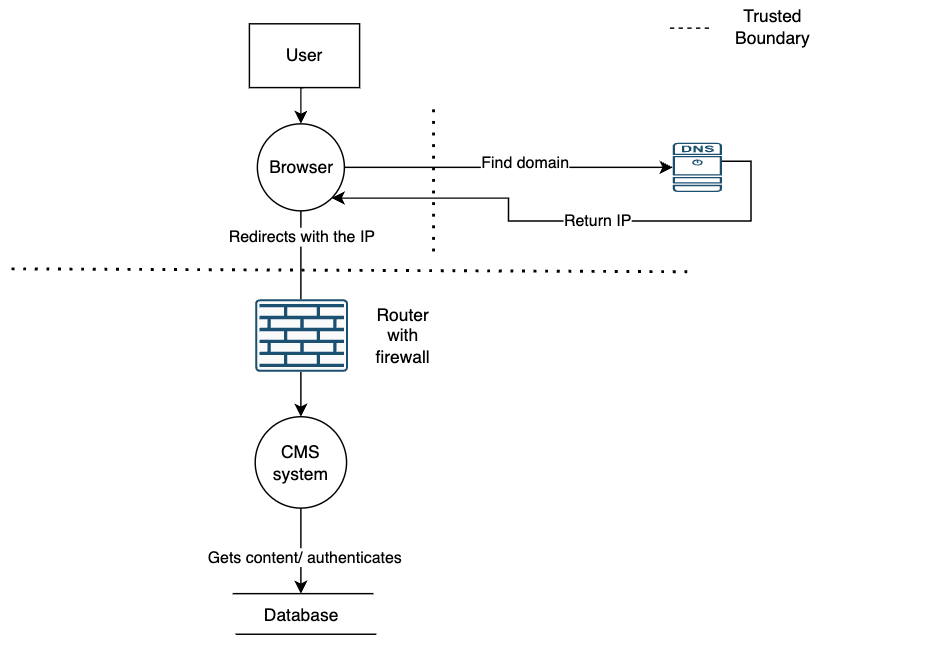
\includegraphics[width=\textwidth, height=280px]{pics/dfd.png}
\caption{DFD level 0 for the CMS system}\label{fig:dfd}
\end{figure}


\section{Vulnerability Assessment}
For the vulnerability assessment, the automated tools (see table \ref{table:tools}) mentioned in the baseline analysis were used to scan for known threats and misconfigurations of the CMS system using the adversary behaviors defined in MITRE Enterprise ATT\&CK matrix \citep[p.~158]{xiong2022cyber}.

\begin{comment}
Additionally, the assessment and reconnaissance are performed using the MITRE Enterprise ATT\&CK matrix \citep{mitre_url}, as this model describes the adversary behaviors that measure the system's resilience at an enterprise level \citep[p.~158]{xiong2022cyber}.
\end{comment}



\begingroup
\centering
\setlength{\tabcolsep}{6.5pt} % Default value: 6pt
\renewcommand{\arraystretch}{1.8} % Default value: 1
\begin{longtable}{ |p{5cm}| p{10cm} |}
\caption{Results from the tools used in the assessment}
    \label{table:tools}
\hline
\rowcolor{grey!15}
\textbf{Tool}  & \textbf{Result}\\
\hline
Metasploit \& Nmap &  
\vspace{-\baselineskip}
\begin{enumerate}
    \item Discovered network misconfigurations.
    \item SSL/TLS scans were carried out for the open ports.
    \item Tested against major CRM threats (i.e., SQL injection, XSS, RCE, Directory traversal).
    \item Wordlist scans for discovering vulnerable paths were executed.
\end{enumerate}\\
\hline
Cmsmap &  
\vspace{-\baselineskip}
\begin{enumerate}
    \item CMS and PHP version was scanned and its vulnerabilities.
\end{enumerate}\\
\hline
DNSrecon &  
\vspace{-\baselineskip}
\begin{enumerate}
    \item Performed reverse lookup and CDN detection.
    \item Performed DNS Zone transfer.
    \item Performed Cache Snooping and DNS Recursion.
    \item Performed Zone walking.
\end{enumerate}\\
\hline
\end{longtable}
\endgroup

\section{GDPR Analysis}
Using the GDPR compliance checklist, the website is evaluated for compliance with GDPR \citep{gdpr_checklist}. Failure to comply with GDPR rules with severe violations can be fined up to 4\% of the total turnover, or €20 million \citep[p.~32]{eu_fines}. Table \ref{table:gdpr} summarizes the discovered GDPR compliance results for the CMS system.


\begingroup
\centering
\setlength{\tabcolsep}{6.5pt} % Default value: 6pt
\renewcommand{\arraystretch}{1.8} % Default value: 1
\begin{longtable}{ |p{3cm}|p{5cm}| p{7cm} |}
\caption{GDPR Assessment}
    \label{table:gdpr}
\hline
\rowcolor{grey!15}
\textbf{Article GDPR} & \textbf{Name}  & \textbf{Status}\\
\hline
Art.3 & Representative of Controller in the European Union  &
\vspace{-\baselineskip}
\begin{enumerate}
    \item A representative in the European Union is required as the CRM is hosted in the United States and processes personal data. The presence of the officer is unknown.
\end{enumerate}\\
\hline
Art.12 & Transparent privacy policy use, with the subject's consent.  &  
\vspace{-\baselineskip}
\begin{enumerate}
    \item A consent layer for informing users of the information the cookies collect is missing.
    \item Granular consent is also not present.
    \item Privacy policy of the website link is not present.
\end{enumerate}\\
\hline
Art.25 & Data Protection by Design and default.  &  
\vspace{-\baselineskip}
\begin{enumerate}
    \item The databases containing personal data are available on the public internet, creating a risk of personal data breaches.
    \item The accounts are protected with an authentication mechanism.
\end{enumerate}\\
\hline
Art.32 & Security of Processing.  &  
\vspace{-\baselineskip}
\begin{enumerate}
    \item Unencrypted email servers with ports (110, 143, 465, 587, and 2525) are used and are susceptible to man-in-the- middle-attacks.
    \item The CRM website uses TLS-encrypted connections for data exchange. Unencrypted ports, i.e., 80 and 8080, are redirected to encrypted ones.  
\end{enumerate}\\
\hline
Art.33 \& 34 & Notification of breaches.  &  
\vspace{-\baselineskip}
\begin{enumerate}
    \item Logging and monitoring to detect unusual behaviors are required but cannot be confirmed.
    \item Incident response within 72 hours of a breach is required but cannot be confirmed.
\end{enumerate}\\
\hline
Art.38 & Presence of Data Protection Officer.  &  
\vspace{-\baselineskip}
\begin{enumerate}
    \item A data protection officer handling critical breach incidents is required. The availability of the DPO is unknown.
\end{enumerate}\\
\hline
\end{longtable}
\endgroup
After evaluating the CMS system with the GDPR directive (see Table \ref{table:gdpr}), it can be concluded that significant shortcomings are present in the system, which break the GDPR directive, as many required features like privacy policy, cookie consent, data protection are not adequately implemented and the company can be fined for not them.

\section{CIS Analysis}
An evaluation of the CIS v8 framework is a set of recommended actions to prevent common attacks on networks and systems. This framework is chosen as it prioritizes a simple list of steps in comparison to other frameworks, which can be easily implemented also by small and medium-sized organizations with a low budget \citep[p.~59]{CIS}. Table \ref{table:cis} summarizes the evident shortcomings of the system according to the CIS control safeguards.

\begin{comment}
    
    \begin{figure}[h!]
    \centering
    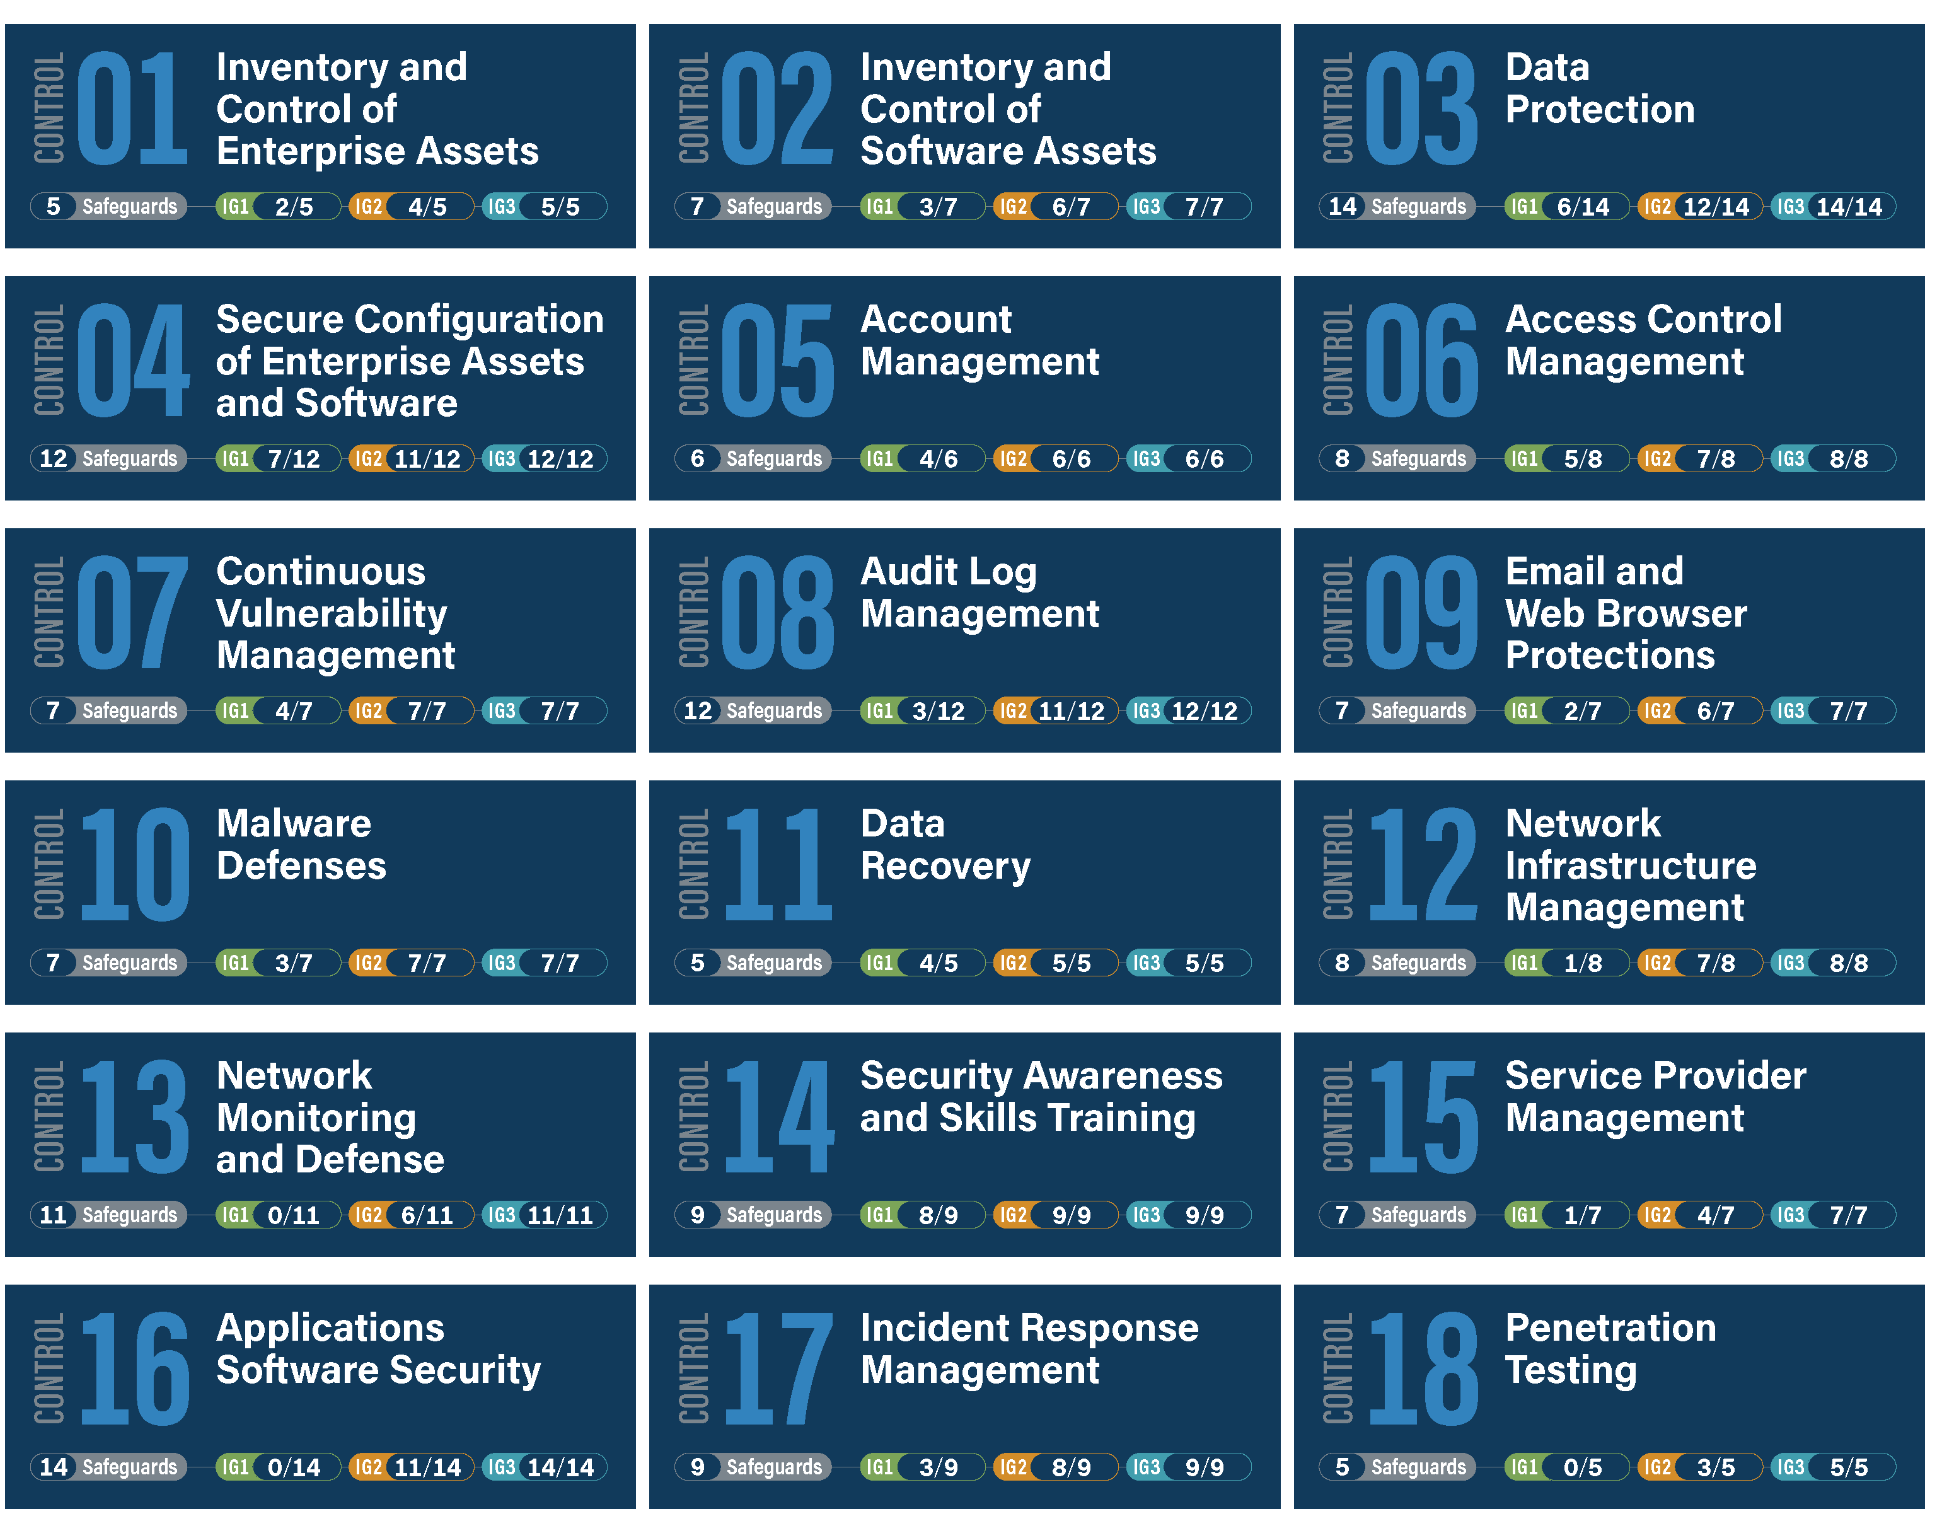
\includegraphics[width=\textwidth]{pics/cis_steps.png}
    \caption{(source:https://www.cisecurity.org/controls/implementation-groups/ig3) CIS Controls}\label{fig:bar_risks}
    \end{figure}

\end{comment}

\newpage
\begingroup
\centering
\setlength{\tabcolsep}{6.5pt} % Default value: 6pt
\renewcommand{\arraystretch}{1.8} % Default value: 1
\begin{longtable}{ |p{7cm}| p{8cm} |}
\caption{CIS Controls}
    \label{table:cis}
\hline
\rowcolor{grey!15}
\textbf{CIS Control}  & \textbf{Status}\\
\hline
Inventory and Control of Enterprise Assets  &  
\vspace{-\baselineskip}
\begin{enumerate} 
    \item Unauthorized assets like databases and FTP servers are not checked regularly, as they are open to the public.
\end{enumerate}\\
\hline
Inventory and Control of Software Assets  &  
\vspace{-\baselineskip}
\begin{enumerate}
    \item Not all software components, i.e., DNS servers and databases, are up-to-date.
    \item It is unclear if a list of authorized software that can be used exists.
\end{enumerate}\\
\hline
Data Protection  &  
\vspace{-\baselineskip}
\begin{enumerate}
    \item Mail and FTP servers do not use encryption in transit.
\end{enumerate}\\
\hline
Network Infrastructure Management  &  
    \vspace{-\baselineskip}
    \begin{enumerate}
        \item Network infrastructure is not up-to-date, i.e., the DNS server is outdated and contains many vulnerabilities.
    \end{enumerate}\\
\hline
\end{longtable}
\endgroup

\section{Limitations}
The assessment consisted of a few constraints as the project. The following limitations were encountered during the vulnerability assessment.
\begin{enumerate}
    \item Evaluating against the frameworks, the points requiring internal organizational knowledge could not be verified, i.e., backups exist, data encryption at rest, the presence of Logs and SIEM, presence of data protection officers. Herefore, the system could only be evaluated partially. 
    \item Some GDPR articles concerning Right to Access, Correct, and Erase Data cannot be evaluated, as we do not have access to any valid user. 
    \item On-site assessments could not be done, as the data centers are physically out of reach for us.
    \item All intrusive testing to verify the found exploits could not be carried out, as there are no legal permissions to attack the system, leading to only assumptions about the blast radius of the vulnerabilities.
\end{enumerate}